\documentclass[12pt]{report}

\usepackage{amsmath, amsfonts}
\usepackage{graphicx}
\usepackage{enumitem}
\usepackage{tikz}
\allowbreak

\newtheorem{definition}{Definition}


\title{\textbf{Engineering Mathematics}}
\author{F17/2054/2022}
\date{November 5, 2023}
\begin{document}

\maketitle

\chapter*{Basic mathematical Concepts}

\section*{Sets}
    \begin{definition}
        A set is a well defined collection or group of objects.
    \end{definition}
    \text{These objects are also referred to as members of a set}
    \begin{enumerate}
        \item Requirements of a set \\
            \begin{enumerate}
                \item A set must be well defined, i.e, must not leave room for any ambiguity.
                \item The elements of a given set must be distinct, i.e, each element should appear only once.
                \item The order of representing elements of a set is immaterial, different arrangement of the \\
                same elements does not showany difference.
            \end{enumerate}
        \item Specifying or naming of sets \\
            \text{By convention, sets are specified (named) using a capital letter. Further, the elements of a set} \\
            \text{are designated by either listing all the elements or by using a descriptive characteristic or pattern.} \\
            \text{The elements of a set are enclosed using curly brackets. We can represent them in three ways:}
            \begin{itemize}
                \item[$-$] Listing of all elements \\
                $ A = \{0,1,2,3,4,5,6\}$
                \item[$-$] Using a descriptive characteristic \\
                $ A = \{\textit{A such that X is a positive integer from 0 to 6 inclusive} \} $
                \item[$-$] Using a pattern \\
                $ A = \{1,2,\ldots,6\}$
            \end{itemize}
        \item Set membership \\
            \text{This is  expressed by using the symbol $\in$. Considering set \textit{A} in which 3 is a member}
            \text{Expressed as 3 \(\in\) \textit{A}}
        \item Finite set \\
            \text{A set that consists of a limited or countable number of elements.}
        \item Subset \\
            \text{Any set \textit{S} is a subset of set \textit{A} if all elements in \textit{S} are members of \textit{A} and is denoted} \\
            \text{by $\subset$ and is read as "\textit{S} is a subset of \textit{A}"} \\
            \text{A is said to be the superset of S denoted by $\supset$, $A \supset S$}
        \item Equality of Sets \\
            \text{If all elements in set D1 are in D2 and all the elements in D2 are in D1 then they are equal D1 = D2}\\
            \text{Can be denoted as $D1 \supset D2 \text{or} D2 \subset D1$, i.e, they are subsets or supersets of each other.}
        \item Universal Set \\
            \text{Set that contains all the elemnts under consideration,denoted U.}
        \item Null or empty set \\
            \text{Is a set with no elements and is denoted by \{\} or $\emptyset$.}
        \item Complement of a set \\
            \text{Given U and $A \subset U$ then the complement of A, denoted by A' or $A^c$ represents all elements} \\
            \text{in U that are not in A.}
        \item Seys are pictorially represented using Venn Diagrams \\
            \text{ }\\
            \textbf{Symbols} \\
            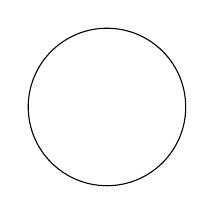
\begin{tikzpicture}
                \draw (0,0) circle(10mm);
            \end{tikzpicture} \\
            \text{ }\\
            \text{Circles: used to represent ordinary sets}\\
            \text{ }\\
            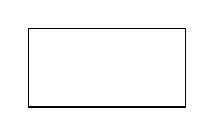
\begin{tikzpicture}
                \draw (0,0) -- (2,0) -- (2,1) -- (0,1) --cycle;
            \end{tikzpicture}\\
            \text{ }\\
            \text{Rectangle: Used to represent Universal set}\\
        \item Singleton Set \\
            \text{Set with only one element}
        \item Disjoint sets \\
            \text{Are two sets with no elements in common}
    \end{enumerate}

\section*{Set Operations and Algebra}
    \begin{definition}
        \text{These are operations where sets are combined to obtain other sets of interest}
    \end{definition}

    \text{Given two sets P and Q}\\

    \text{They include:}\\
    \begin{enumerate}
        \item \textbf{Union of Sets, $\cup$} \\
            \text{Consists of elements in P or Q or both}
            \begin{figure}[h!]
                \includegraphics[width=0.4\linewidth]{union.png}
            \end{figure}
        \item \textbf{Intersection of sets, $\cap$} \\
            \text{Consists of elements in both P and Q(common elements)}
            \begin{figure}[h!]
                \includegraphics[width=0.4\linewidth]{intersection.png}
            \end{figure}
        \item \textbf{Set difference/Injunction, $\setminus$} \\
            \text{Consists of elements in P but not in Q}
            \begin{figure}[h!]
                \includegraphics[width=0.4\linewidth]{set_difference.png}
            \end{figure}
        \item \textbf{Symetric difference, $\Delta$} \\
            \text{Consists of elements in P but not in Q and thos in Q but not in P}
                \begin{figure}[h!]
                    \includegraphics[width=0.4\linewidth]{symmetric_diff.png}
                \end{figure}
    \end{enumerate}

\section*{Laws of Set aAlgebra}
    \begin{enumerate}
        \item Commutative Laws \\
            \text{The order in which sets are combined in union or intersection is irrelevant, i.e}
            \text{$P \cup Q = Q \cup P$ and $P \cap Q = Q \cap P$}
        \item Associative Laws \\
            \text{The selection of 3 or more sets for grouping in a union or intersection is immaterial, i.e}
        $(P \cup Q) \cup R = P \cup (Q \cup R)$
        \item Distributive Laws \\
            \text{For any 3 sets P, Q and R:}\\
        $P \cup (Q \cap R) = (P \cap Q) \cap (P \cup R)$        
        \item Impotent Laws \\
            \text{For a set Q}\\
            $Q \cup Q = Q$ \text{and} $Q \cap Q = Q$\\
            \textbf{Other Laws: } \\
        \item $P \cup \emptyset = P$ \\
        \item $P \cap \emptyset = \emptyset$ \\
        \item $P \cup U = U$ \\
        \item $P \cap U = P$ \\
        \item $P \cup P' = U$\\
        \item $P \cap P = \emptyset$\\
        \item De Morgan's Laws\\
            \text{For  any two sets Q and R}\\
            \begin{itemize}
                \item[i] $(Q \cup R)' = Q' \cap R'$
                \item[ii] $(Q \cap R)' = Q' \cap R'$
            \end{itemize}
    \end{enumerate}
\section*{Boolean Algebra}
    \text{Can be used to describe the manipulation and processing of binary information}\\
    \text{It's two-valued and has applications in the design of modern computer systems.}\\
    \text{It is common to inteprete the digital values 0 as false and 1 as true.}\\
    \textbf{Definitions}\\
    \begin{enumerate}
        \item 
    \end{enumerate}
    

\chapter*{Cartesian Products and Relations}

\text{For two sets \textit{A} and $B$, the Cartesian Product of \textit{A} and $B$ is\\}
$$A \times B = \{(a, b); a \in A, b \in B\}$$
\text{We say that the elements of \textit{A} \(\times\) $B$ are ordered pairs\\}

\begin{definition}
: For sets A, B, any subset of \textit{A} \(\times\) $B$ is called a binary relation from
\textit{A} to $B$. Any subset of \textit{A} \(\times\) \textit{A} is called a \textbf{binary relation} on \textit{A}.
\end{definition}
\end{document}